\section{Introduction}
\label{sec:introduction}

%% What are soft actuators, why are they useful?
\David{You might want to split these two questions into two paragraphs: What are soft actuators? why are they useful?}
\David{ As a writing tool, I would suggest to give paragraphs titles in latex comments.  Those titles should form a story.}
\David{I'm not sure if the reference to Biology is necessary in this first sentence.  It might give the paper a spin that you don't intend.}
Soft continuum manipulators, resembling biological trunks and tentacles, offer capabilities beyond the scope of traditional rigid link manipulators. Namely, their compliant structure allows them to adapt their shape to navigate unstructured environments, safely work alongside humans, and absorb large impacts without damage. A central feature of continuum manipulators is continuously deformable backbones in place of rigid links connected by discrete joints. In order to utilize this feature effectively, actuation methods are needed for continuum manipulators that do not inhibit their compliance.

%% Extrinsic vs. intrinsic actuation
\David{Reading this and the next paragraphs felt a little bit like a detour.  You introduce these two concepts to achieve at the conclusion that a FREE is combining benefits of both.  It reads a bit like you are constructing this case.  Some people might disagree with this classification (there is not citation to support it with literature) and then they won't follow with your conclusions.}
\David{I would propose a more ``positive'' approach in which you don't talk about disadvantages of other systems (this makes you vulnerable for two reasons 1) you piss off people 2) you would need to cover everything else that exists to make your case) but instead just highlight the advantages of yours.}
\David{After starting with one-two paragraph(s) that briefly introduce what soft robots are and why they are useful, I would suggest to focus on fluid-powered systems: ``A large number of soft robotic system are driven by fluid powered actuators \cite{}.  In these actuators, pressurized fluid such as water or air creates a targeted deformation of a soft structure that surrounds a fluid filled cavity.  To achieve a specific type and direction of deformation, and not merely a homogeneous expansion, the stiffness of the soft structure is pattered in a specific way, either by the use inhomogeneous materials \cite{} or by adding reinforcing elements such as fibers, beams, or plates \cite{}.  Examples of these actuators include bellows \cite{,} McKibben muscles \cite{}, ...\cite{}, or ... \cite{}.  The big advantage of these actuators is that they are inherently soft and thus carry all the benefits of soft robotic systems.''}
Current continuum manipulators utilize one of two actuation approaches, intrinsic or extrinsic. Intrinsically actuated manipulators have actuators mounted directly to their backbone, producing forces locally. Soft fluid-driven actuators such as bellows (cite) or McKibben muscles (cite) are popular choices for such schemes due to their ability to produce forces without imposing structure (cite octarm, festo). Extrinsically actuated manipulators, on the other hand, have actuators located off of the manipulator arm itself, and transfer forces to the arm via cables (cite). A benefit of this approach is that it can rely on more conventional actuators such as motors. 

%% Downsides of each type
\David{I would remove this `downside' paragraph it is hard to make it complete.  Instead, focus on the advantages of FREEs}
One downside of intrinsic actuation schemes is that the direction of the forces applied cannot be redirected arbitrarily, since the actuators are mounted directly to the backbone. For this reason, most intrinsically actuated continuum manipulators are adept at producing bending moments, but not twisting. Extrinsic actuation schemes do better in this regard, as cables can be routed and attached to the backbone in ways that produce both bending and twisting moments (cite Clemson, surgical robots). However, cable driven schemes introduce complications such as slack and backlash, which typically require complex mechanical or control systems to remedy \cite{walker2013continuous}.

%% What is a FREE and why it is great.
\David{So rather than saying what the disadvantages of other systems is, focus on why FREEs are good:}
\David{``A particularly promising type of soft fluidic actuators are fiber reinforced elasomeric enclosures (FREEs).  In these actuators an elastomeric fluid-filled tube is wound with reinforcing fibers that pattern the stiffness of the actuator to yield a desired mode and direction of deformation (figure????).  By changing the number, type, and angle of these fibers, FREEs can be customized to yield a large variety of desired deformations.  In particular, for FREEs with a single set of equally wound fibers, changing the angle of the fiber wrapping yields uniquely different combinations of axial forces and twisting torques.''}
The fiber reinforced elasomeric enclosure (FREE) is a type of fluid driven soft actuator that combines the simplicity of intrinsic actuation with the versatility of extrinsic actuation. Composed of an elastomeric tube wound with fibers, FREEs simultaneously exert forces along their central axis as well as moments about that axis \cite{bishop2015design} (see Figure \ref{fig:FMratios}b). This enables FREEs mounted directly to a compliant backbone to produce both bending and twisting moments, without introducing complications like slack or backlash. \David{Not sure if you need the notion of a backbone here...} The ratio between the force and moment produced by a FREE is also customizable, determined by the angle of the wrapped fibers. This unique property of FREEs can be exploited in the design of parallel configurations to generate arbitrary forces at an end effector.

%% The question:  How to combine them in parallel???
\David{I would add a paragraph that discusses the question that you try to answer.}
\David{`` Given that a single-fiber-family FREE essentially only represents }


%% Existing literature.
Until now, the literature regarding fiber-reinforced fluid-driven actuators has focused mainly on their kinematics \cite{bishop2015design, bishop2012parallel, connolly2015mechanical} or on the forces generated by single actuators \cite{bruder2017model, sedal2017constitutive}. In this paper, we present a novel way to calculate the forces in terms of a state dependent Jacobian matrix and input pressure. We then extend this model to predict the forces generated by parallel combinations of FREEs in arbitrary parallel configurations, and validate the model by comparing its predictions to those measured on a physical system. By characterizing the way parallel combinations of FREEs generate forces, this work lays the foundation for future applications, including actuation of continuum manipulators.
%, then consider the possible sources of error. This work lays the foundation for future application including the use of FREEs to actuate continuum manipulators.
%We conclude with a discussion of the potential benefits and challenges of using FREEs to actuate continuum manipulators.


% In this paper we define an object called the ``force polygon'' as the set of all possible forces that can be generated by a parallel combination of actuators at an end effector. This object provides a way of comparing the relative effectiveness of different parallel combinations in generating forces, in that the dimension of the force polygon corresponds to the end effector's number of actuatable degrees of freedom. 

% For example, the McKibbon actuators used in the Octarm robot produce large contractile forces but little resistance to bending, enabling curvature along the length of the entire arm (cite). 



\section{Fiber Angle and the Force/Moment Ratio}

The ratio between the force and the moment generated by a FREE is determined by the nominal fiber angle, $\Gamma$ (Figure \ref{fig:FREEparams}). To understand why this is the case, consider a cable being pulled in a plane (Figure \ref{fig:FMratios}a). The angle between the cable and the y-axis determines the magnitude of the components of the cable force along the x and y directions. The ratio between the components in the x and y directions is simply
\begin{align}
    \frac{T_x}{T_y} &= -\cot{\Gamma}     
\end{align}
%Similarly, the fibers in a FREE are loaded in tension by the internal fluid pressure, and the components of that tension are determined by the fiber angle (Figure \ref{fig:FMratios}). The components of fiber tension in the rotational and axial directions then contribute to the total torque and axial force of the FREE, as derived and explained in \cite{bruder2017model}. Since fluid pressure is used to load tension in the fiber (rather then a motor/pulley or something similar) the expressions for force and torque in terms of fiber angle are slightly more complicated than in the planar cable example, yielding the following expression for the force/moment ratio of a FREE in its undeformed state
Similarly, the fibers in a FREE are loaded in tension. Since fluid pressure is used to induce this fiber tension (rather then a motor/pulley or something similar) the expressions for force and moment in terms of fiber angle are slightly more complicated than in the planar cable example, as derived and explained in \cite{bruder2017model}
\begin{align}
    \frac{F}{M'} &= \frac{1 - 2 \cot^2{\Gamma}}{2 \cot{\Gamma}}
\end{align}
where $M' = \frac{M}{r}$. Figure \ref{fig:FMratios} illustrates that with a suitable choice of fiber angle $\Gamma$ and radius $r$, a FREE can be constructed with an arbitrary force/moment ratio. It should be noted, however, that as $\Gamma$ approaches $90^\circ$, the magnitudes of force and moment per unit pressure decrease significantly. While it is technically possible to choose $\Gamma$ to produce any desired force/moment ratio, FREEs with lower $\Gamma$ values generate forces much more effectively than those with higher $\Gamma$ values. This implies that FREEs are generally better at producing contractile forces than extensile forces.

\begin{figure}
\centering

\begin{tikzpicture} %[every node/.style={draw=black}]
% \draw[help lines] (0,0) grid (4,2);
\matrix [row sep=0cm, column sep=0cm, style={align=center}] (my matrix) at (2,1)
{
\node[style={anchor=center}] {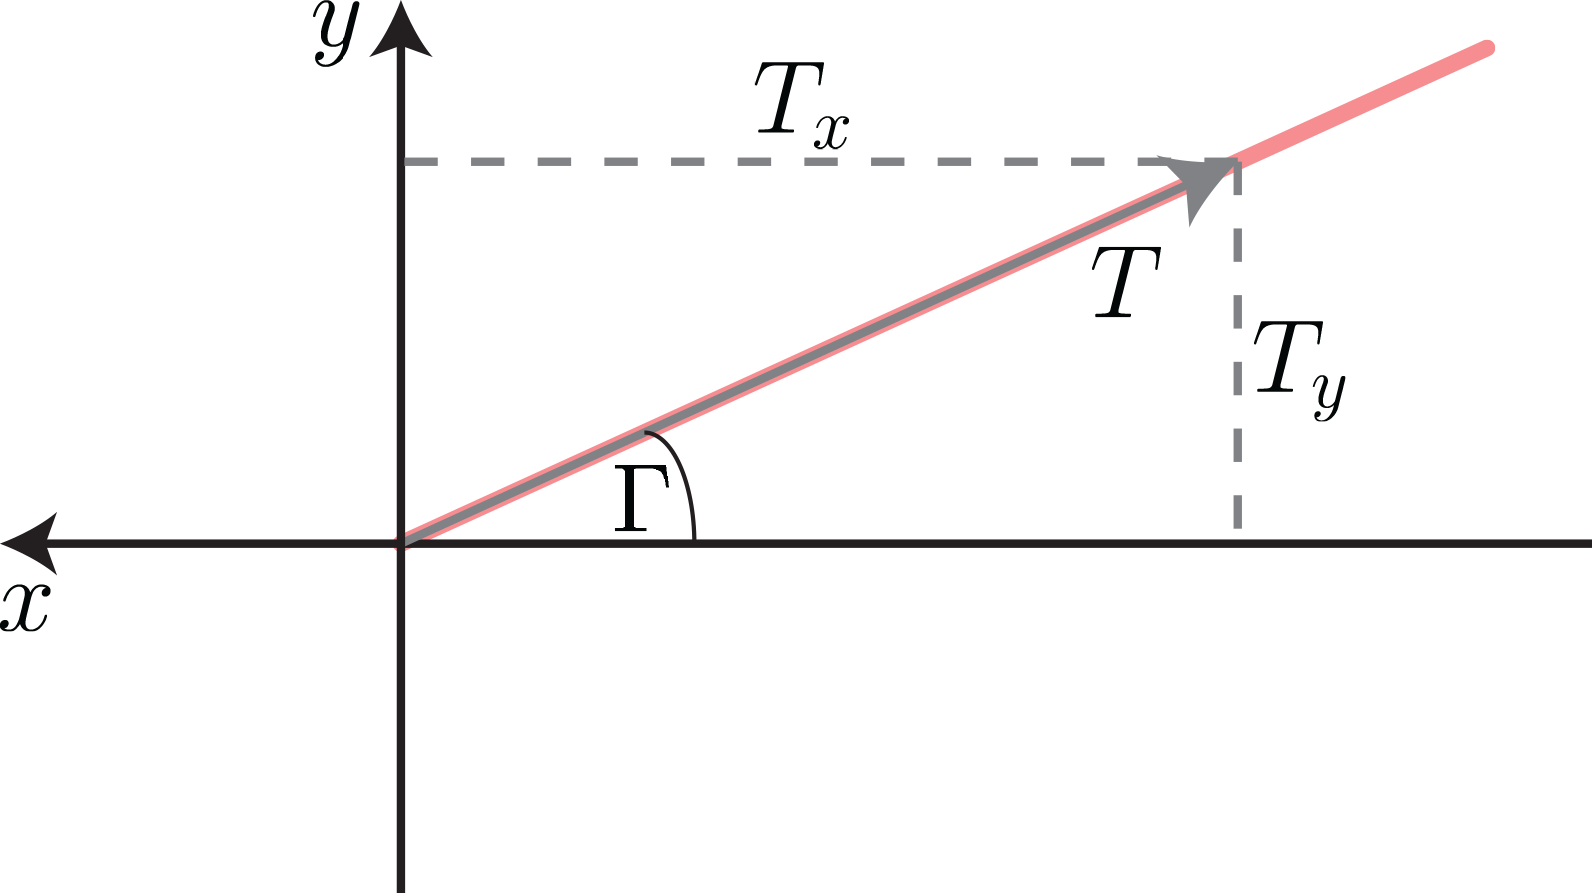
\includegraphics[width=0.42\linewidth]{figures/cableTension.png}}; %\fill[blue] (0,0) circle (2pt);
&
\node[style={anchor=center}] {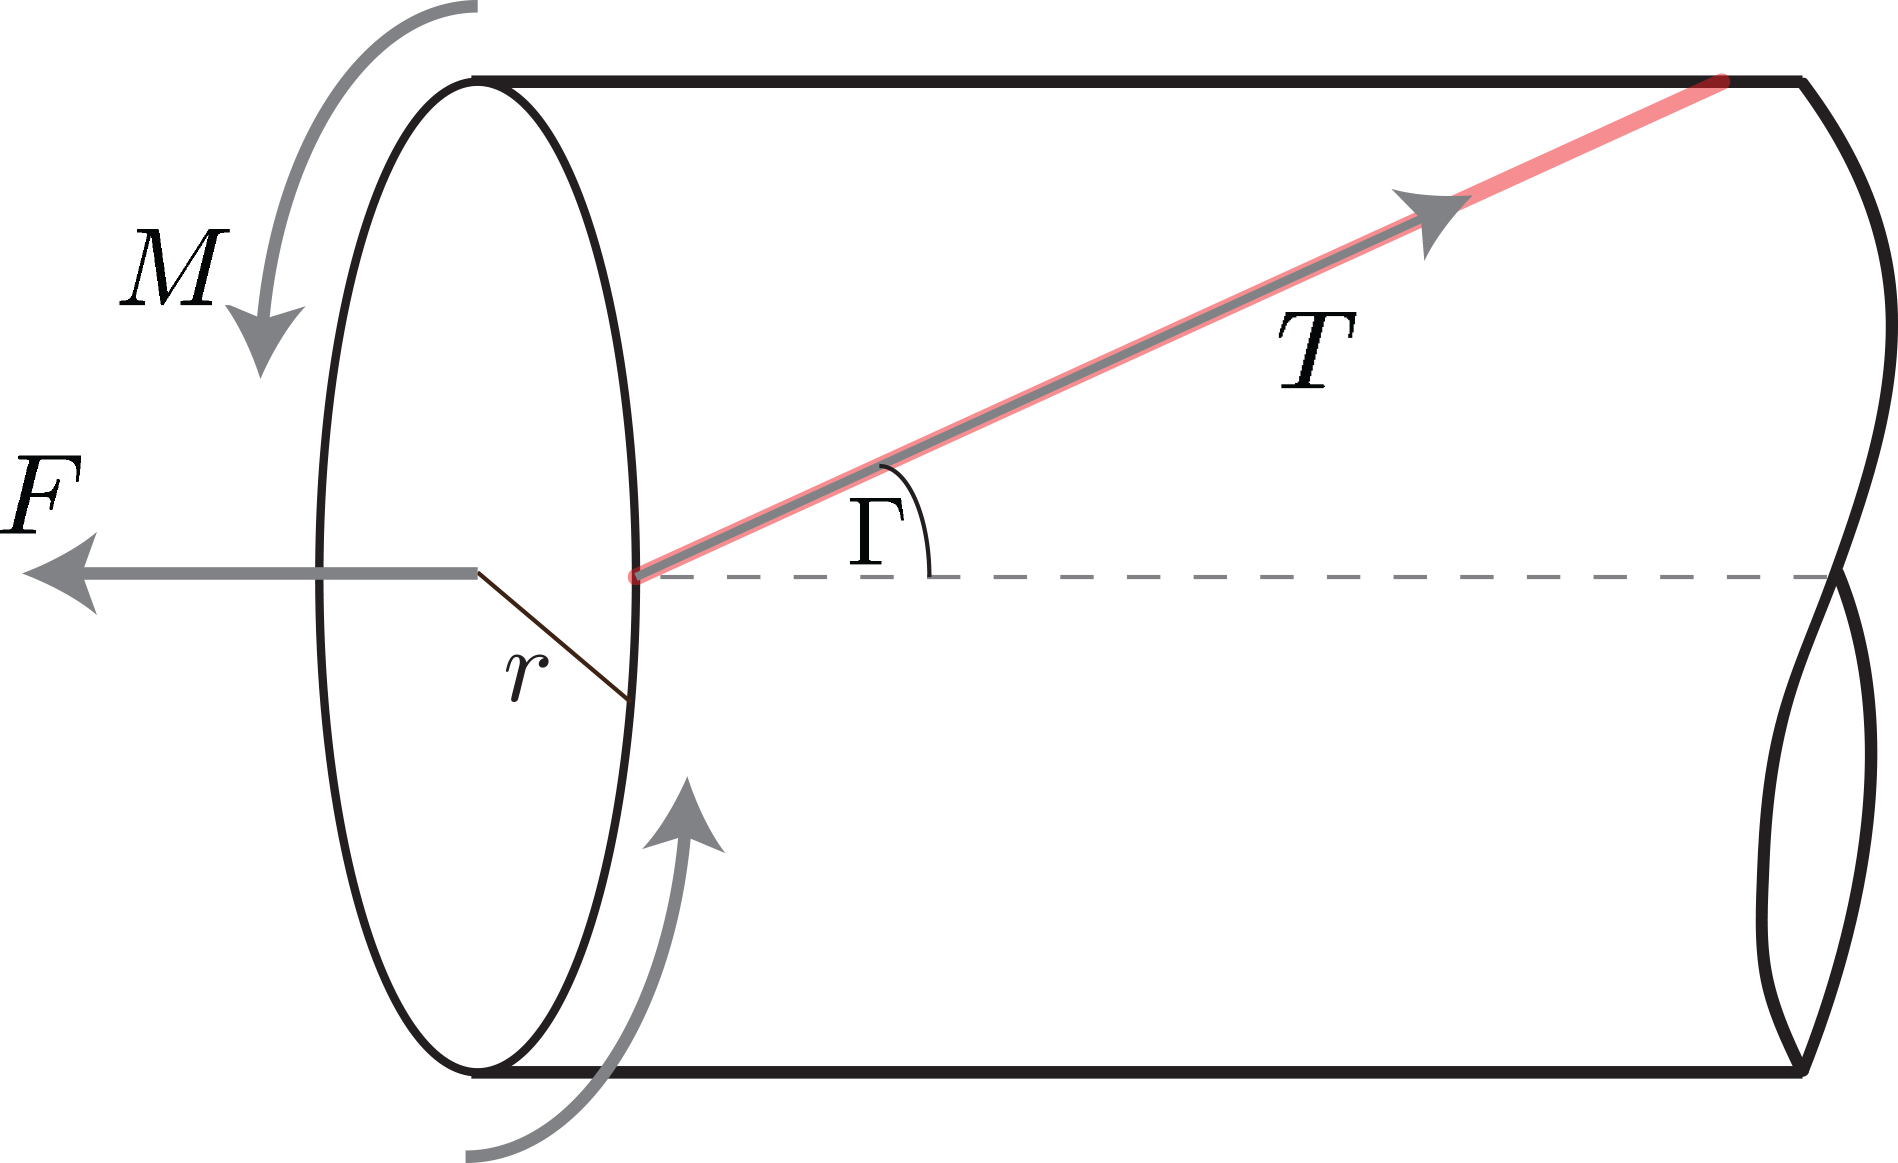
\includegraphics[width=0.42\linewidth]{figures/fiberTension2.png}}; %\fill[blue] (0,0) circle (2pt);

\\
\node (a) {(a)}; & \node (c) {(c)};
\\

\begin{axis}[
    xlabel={\footnotesize{$\Gamma$}},
    ylabel={\footnotesize{$T_x/T_y$}},
    ymin=-10, ymax=10, ytick={0}, ylabel near ticks,
    xmin=0, xmax=90, xtick={0,90}, xticklabel=$\pgfmathprintnumber{\tick}^\circ$, xlabel near ticks,
    tick label style={font=\footnotesize},
    width=0.5\linewidth,
    anchor=center,
]
    \addplot [domain=0:90, dashed] {0};
    \addplot [domain=1:90, samples=100] {-cot(x)};
\end{axis};
& 
\begin{axis}[
    xlabel={\footnotesize{$\Gamma$}},
    ylabel={\footnotesize{$F/M$}},
    ymin=-10, ymax=10, ytick={0}, ylabel near ticks,
    xmin=0, xmax=90, xtick={0,54.7,90}, xticklabel=$\pgfmathprintnumber{\tick}^\circ$, xlabel near ticks,
    tick label style={font=\footnotesize},
    width=0.5\linewidth,
    anchor=center,
]
    \addplot [domain=0:90, dashed] {0};
    \addplot [domain=1:90, samples=100] {(1-2*cot(x)^2) / (2*cot(x))};
    \addplot [mark=none, dashed] coordinates {(54.7,-10) (54.7,10)};
\end{axis};
%\fill[blue] (0,0) circle (2pt);

\\
\node (b) {(b)}; & \node (d) {(d)};
\\
};
\end{tikzpicture}

\caption{By changing the fiber angle of a FREE, it can be configured to produce a large range of force/torque combinations. To understand this, we consider how (a) the angle at which a fiber is pulled in a plane affects (b) the ratio between the $x$ and $y$ components of the pulling force. Similarly, by (c) wrapping the plane into a cylinder and accounting for an internal pressure force pushing out on the endcap, the (d) ratio between axial force and twisting moment can be arbitrarily set by changing the fiber angle.}
\label{fig:FMratios}
\end{figure}